
\documentclass[10pt]{article}
\usepackage[final]{graphicx}
\usepackage{amsfonts}
\usepackage{url}
\usepackage{mathtools}
\usepackage{amsmath,amsthm,amssymb}
\usepackage{subcaption,bm} 
\usepackage{float}


\topmargin -.5in
\textwidth 6.6in
\textheight 9in
\oddsidemargin 0in
\usepackage{color}
\newcommand{\arvind}[1]{{\color{red}{Arvind: {#1}}}}
\DeclarePairedDelimiter\norm{\lVert}{\rVert}
\def\PM{{\mathrm{PM_{2.5}}}} 

\def\ds{\displaystyle}
\def\d{\partial}
\linespread{1.5}

\newcommand{\alennote}[1]{{\color{green}{Alen: {#1}}}}
\newcommand{\kelly}[1]{{\color{blue}{Kelly: {#1}}}}

\begin{document}

\centerline{\large \bf Fusing surface and satellite-derived PM$_{2.5}$ observations to determine the impact } 

\centerline{\large \bf of international transport on coastal PM$_{2.5}$ concentrations in the western U.S.}

\vspace{.1truein}

\def\thefootnote{\arabic{footnote}}
\begin{center}
  Neha Bora\footnote{Department of Mathematics, Iowa State University},
  Tuo Chen\footnote{Department of Statistics, University of Florida},
  Dana Cochran\footnote{Department of Mathematics, California State University Channel Islands},
  Kelly Dougan\footnote{Department of Mathematics, The State University of New York at Buffalo},
  Gautam Sabnis\footnote{Department of Statistics, Florida State University},
  Chuanping Yu \footnote{Industrial and System Engineering, Georgia Institute of Technology}
\end{center}

%\vspace{.1truein}

\begin{center}
Mentors: Alen Alexanderian\footnote{North Carolina State University},
Brett Grant\footnote{Environmental Protection Agency},
Elizabeth Mannshardt\footnote{Environmental Protection Agency}, 
Jessica Matthews\footnote{National Oceanic and Atmospheric Administration}
Arvind Saibaba\footnote{North Carolina State University}.

\end{center}


\vspace{.3truein}
\centerline{\bf Abstract}

Long term exposure to PM$_{2.5}$ is associated with human health complications. Surface readings of PM$_{2.5}$ in the states on the West Coast of the United States have reported to be higher than allowed by the Clean Air Act. One possible reason for this is international transport of air pollution on PM$_{2.5}$. This project explores the relationship between the surface readings of PM$_{2.5}$ from coastal sites with the AOD measurements from the AVHRR in these regions. Once we found a correlation between these readings, we implemented a model to approximate PM$_{2.5}$ concentrations in the Pacific ocean, where surface readings are not possible. We model the variability in PM$_{2.5}$ concentrations using a Generalized Additive Model (GAM) 

\section{Introduction}
%start with info on PM$_{2.5}$ and AOD - definition, how they are monitored and that they measure harmful pollutants

Domestic sources of emissions are the primary cause of air pollution in the
US. However, the international flow of air pollution into
the US could potentially be a contributing factor in some coastal cities with 
high measurements of air pollution. The impact of international transport of
air pollution on our ability to attain air quality standards or other
environmental objectives in the US has yet to be fully understood. In
other words, cities in the western US may unknowingly be receiving high
pollutant values from external sources. {To answer such questions, 
we need a comprehensive understanding of the transport in the
atmosphere.  }



{We focus on two different measures of pollution, namely PM$_{2.5}$ and Aerosol
Optical Depth (AOD).} PM$_{2.5}$ is particulate matter that is less than $2.5$
micrometers in diameter and is often referred to as the greatest health risk of
pollutants~\cite{epa}. For this project, we used two different sources of data: 
{AOD} measurements obtained from the Advanced Very High Resolution
Radiometer (AVHRR) satellite measurements, and surface PM$_{2.5}$ measurements.
AOD measurements refer to a quantitative measure of the amount of light that is
obstructed by particles in the atmospheric column and are also referred to as
aerosol optical thickness (AOT). Because AOD measures any particle from the
satellite to the earth's surface, the measurements of the amount of the
specific pollutant PM$_{2.5}$ are, for the most part, measured by ground sites.

\paragraph{Previous work} Several previous studies have attempted to find
correlations between PM$_{2.5}$ readings and AOD readings. Liu et al  looked
into estimating PM$_{2.5}$ concentrations using the satellite AOD data,
meteorology, and land use information in states surrounding
Massachusetts~\cite{liu}. In their study, they were able to predict PM$_{2.5}$
values better with an AOD model than with a non-AOD model. Lee et al developed
a novel approach in which he used a mixed effects model to predict day-specific
PM$_{2.5}$ concentrations based on AOD measurements~\cite{lee}. Li et
al~\cite{li} investigated if variability of AOD measurements can be used to
infer space-time variability of PM$_{2.5}$ readings. Their model resulted in good
spatial agreement in the eastern region but not the central or western regions
of the US. Overall, they concluded that the relationship between PM$_{2.5}$ and AOD
varies over different locations and times, and that a better prediction model
would be one that focuses on a smaller region or time frame. Van Donkelaar et al (2015) looked for global trends of PM$_{2.5}$
concentrations from satellite data. Using a decadal mean over the years
2001-2010, in North America, they found a relatively higher concentration of PM$_{2.5}$
in the east coast and in the San Joaquin valley of California. In Asia, they
found extremely high concentration, over 60 $\mu$ g $/$ m$^3$ and 80 $\mu$ g
$/$ m$^3$ in Northern India and Eastern Asia, respectively. They found that the
population-weighted concentrations in East Asia nearly doubled the global mean.
These studies suggest that AOD-based models can be used to predict PM$_{2.5}$
concentrations on a daily basis, using a statistical model interpolating over a
sufficiently small space and time scale.

\paragraph{Overview of main results} The goal in this project is to establish a
relationship between AOD measurements from the AVHRR satellite and PM$_{2.5}$
measurements. We focus our analysis  on the coasts of California and Hawaii
since at these sites there is a significant overlap between these two datasets.
We aim to use AOD-PM$_{2.5}$ relationship to predict PM$_{2.5}$ concentrations
over the Pacific Ocean. In addition, we analyze time series models of surface
PM$_{2.5}$ measurements at each site. Spatial interpolation is also used on all
PM$_{2.5}$ sites in California to help determine a trend in the readings. These
images were used to visualize high emission events in the state such as
wildfires, dust storms, etc. This analysis makes a significant progress in 
understanding the impact of international transport of air pollution on
PM$_{2.5}$ concentrations in coastal areas of the western US.

\section{The Problem}





\subsection{Description of data}

The first dataset of Climate Data Record (CDR) of AOD was obtained from the
National Oceanic and Atmospheric Administration (NOAA)~\cite{noaa}. 
This data was collected using AVHRR, which is a device that 
detects radiation. The device records 
an optical measure of aerosol column loading derived from the global ocean
pixel-level PATMOS-x AVHRR clear-sky reflectance CDR at $0.63$ $\mu$m
channel~\cite{noaa}. 
This satellite provides global readings of oceanic measurements of AOD for the
years $1981$-$2009$~\cite{noaa}. 
The second dataset, provided by EPA,
contained the surface PM$_{2.5}$ measured in California, Oregon, Washington,
Alaska, and Hawaii.~\cite{epa}.

The AVHRR takes approximately $16$ days to make one revolution around the
earth. We, thus, have roughly two data values for each month of the year at
each pair of coordinates, for the years 1981-2009. The frequency of the
PM$_{2.5}$ data collected from each site varies from once every day to once
every six days. On certain occassions, the measurements from the satellite were
found to be  erroneous due to light reflection from cloud covers. Additionally,
there are times when the PM$_{2.5}$ sensors malfunctioned resulting in no data.
These points were appropriately removed from the datasets. %Hence, we sometimes
have months that have only two or less PM$_{2.5}$ data and/or no AOD data. 

Additionally we have satellite data for wind speed, wind direction, air
temperature, relative humidity, and  height of the planetary boundary layer.
This data was incorporated in our models to give more accurate results. The
wind data was provided into a u wind and v wind format, where u represents wind
blowing towards the east, and v represents wind blowing toward the north. The u
wind needed to be scaled by a factor of $0.003052037$, as indicated in the file
information. The formulas to get the wind speed and the wind direction are
below, where $u_\text{wind}$ and $v_\text{wind}$ represent the u and v values.
\cite{wind}

\[
\begin{aligned}
\text{windspeed} &= \sqrt{u_\text{wind}^2 + v_\text{wind}^2},\\
\text{winddirection} &= \displaystyle\frac{180}{\pi} \arctan(-u_\text{wind}, -v_\text{wind}) + 180.
\end{aligned}
\]

\subsection{Challenges}
One of the challenges with the given data set was its size. For example, the file size for one year of AOD data was 9.47 GB, which exceeded the memory of our systems. Instead of using AOD data for one year in one file, we dowloaded daily AOD data. We restricted our AOD data set to the years 2006-2009, where we had access to the files in daily format. %\kelly{Ask Gautam about these specifics, write in a positive way}We combined the results in MATLAB. This process was a bit time consuming and we thus only received AOD data for the years 2006 - 2009. 

The next challenge was with the format of the latitude and longitude of wind, air temperature, relative humidity, and height of the planetary boundary layer data. The data covered North America and was in the Lambert Conformal Conic map projection. However, the PM$_{2.5}$ and AOD data are in geographical coordinates. The geographical coordinates of the PM$_{2.5}$ sites were converted to Lambert Conformal Conic coordinates in order to extract the values of these meteorological variables. 

The PM$_{2.5}$ sensor readings had some challenges as well. The main issue was
that not all sensor sites pick up measurements on the same day. Thus, if we
wanted to look at sensor readings on say Jan 1, 2008, we may only have 10 sites
that produce measurements, but if we took a look at Jan 2, 2008, we may have 40
sites that produce measurements. Consequently, on many days, we had
insufficient data to construct meaningful spatial interpolations.





\section{The Approach}

\subsection{Data processing}




No matter what PM$_{2.5}$ sites we consider using, we need to find the closest
AOD coordinates to the PM$_{2.5}$ sites. In addition, we need to find dates
when both types of data are available. This requires searching all the
observations in the AOD dataset. 
Additionally, AOD dataset has a lot of missing data, thus we need
to clean the AOD data first.  Since the data we want to use is located on the
west coast,  we used the longitude and latitude of the west coast to eliminate
data from other locations that we will not use. We then dropped all the missing
data and changed the original format of the data into more readable one, where each record 
is of the form~\verb+(date,  latitude, longitude, AOD)+.

%\begin{table}[H]
%%\centering
%\begin{tabular}{|c|c|c|c|}
%\hline 
%Date & lat\_aod & long\_aod & aod\\
%\hline
%2000-01-25 & 30 & -126.6 & -0.0836133733391762 \\
%\hline
%$\cdots$ & $\cdots$ & $\cdots$ & $\cdots$\\
%\hline
%\end{tabular}
%\caption{AOD data.~\alennote{Do you need the second row with all the $\cdots$?}}
%\label{tbl:AOD_data}
%\end{table}


\subsection{PM$_{2.5}$ sites adjacent to AVHRR grids}
Since the coverage of the AOD data is over the oceans and the PM$_{2.5}$ data
is collected over the land, there is no direct overlap between the two
datasets. In order to compare the two data sets, we adopt the following
strategy. First, of all the PM$_{2.5}$ measurement sites, we identify those
that are close to the coast. Figure~\ref{fig:locations} shows the geographical
locations to $13$ locations, most of which lie in California.   In the rest of
this report, we focus on only $2$ site locations. Future work will include
examining the additionally $11$ locations. 

\begin{figure}[H]
\centering
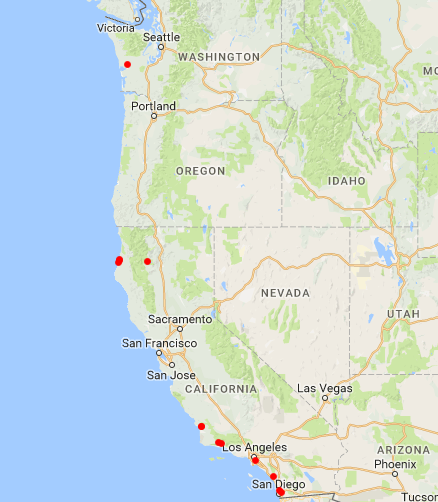
\includegraphics[width=0.5\textwidth]{pm13.png}
\caption{13 sensor sites along West Coast.}
\label{fig:locations}
\end{figure}




\subsection{Analyzing PM$_{2.5}$ trends}
One method we used to analyze trends in the PM$_{2.5}$ data was to make an
animation to show the change in the concentration of PM$_{2.5}$  over time. The
animation plots points at each site where the PM$_{2.5}$ data was collected,
with color varying depending on the intensity of the reading, with darker
colors indicating a larger concentration of PM$_{2.5}$. The animation can be downloaded 
from~\url{https://github.com/gautamsabnis/imsm2016_epa/blob/master/PM_time_series.pdf}.

To understand whether we can use measured PM$_{2.5}$ to predict future
PM$_{2.5}$ values, we conducted a time series analysis. We focus our
attention on the PM$_{2.5}$ site near Long Beach, California, which is located
at latitude 33.79236 and longitude -118.175. We collect monthly averaged
PM$_{2.5}$ values from January 2004 to December 2014, which are plotted in Figure~\ref{fig:time_series}.   

\begin{figure}[H]
\centering
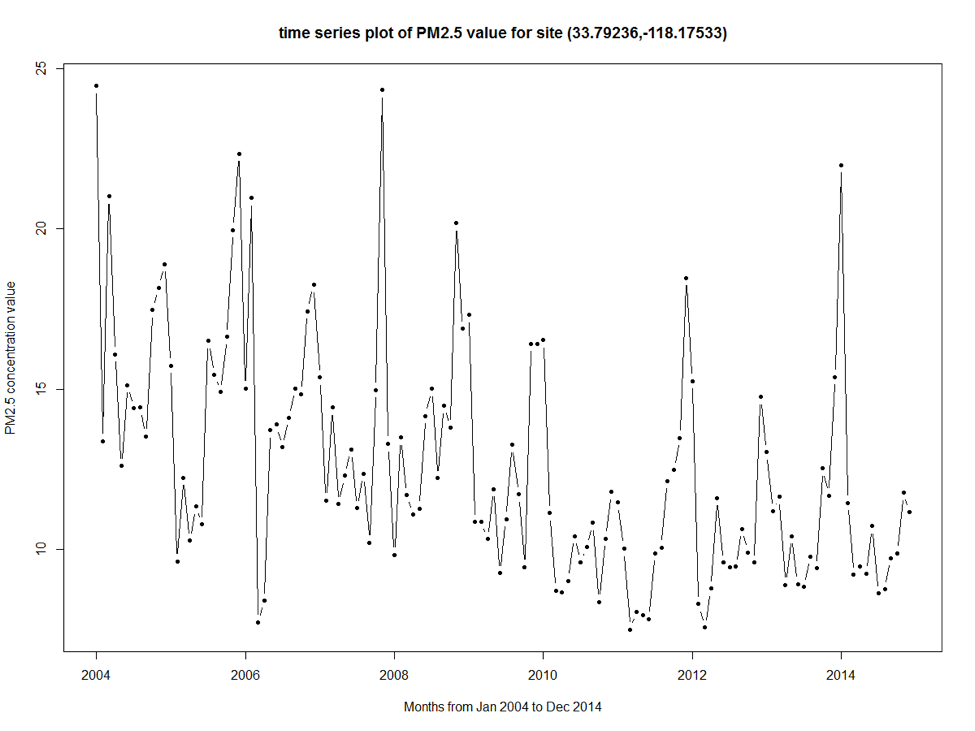
\includegraphics[width = 100mm]{ts1.png}
\caption{Time series plot of PM$_{2.5}$ value for site (33.79236,	-118.17533).}
\label{fig:time_series}
\end{figure}

Figure~\ref{fig:time_series} suggests that there is a slightly 
downward trend over time and the time series seems to exhibit
seasonality. We decided to use two different methods to fit the
time series. One is Holt-Winters Exponential Smoothing. Exponential smoothing
is a very popular scheme to produce a smoothed time series and it assigns
exponentially decreasing weights as the observations get older~\cite{nist}.
Holt-Winters Exponential Smoothing can be used to make short-term forecasts on
a time series that can be described using an additive model with increasing or
decreasing trend and seasonality~\cite{littlebook}. The second method used is the
Autoregressive Integrated Moving Average, (ARIMA). This model can be fitted to
time series data either to better understand the data or to predict future
points in the series~\cite{wik}. 
For the ARIMA method, we first
adjust the time series by subtracting the estimated seasonal component and then
apply the model to the adjusted time series; see Section 4, for the computational 
results. 



%%%%%%%%%%%%%% Maybe the github link for the animation
\subsection{Relationships between AVHRR AOD and surface PM$_{2.5}$}

Our main goal is to explore the relationship between PM$_{2.5}$ measurements obtained from the ground sites and the AOD measurements obtained from the satellite near the coast. We want to ascertain whether satellite remote sensing can be used to assess PM$_{2.5}$ air quality for areas where surface PM$_{2.5}$  monitors are not available. The AOD measurements reflect the integrated amount of particles in the vertical column, and can be used as an input parameter in statistical models for predicting PM$_{2.5}$ levels. Since time-varying parameters such as relative humidity, wind direction, wind speed and air temperature can influence the PM$_{2.5}$-AOD relationship, we want to formulate a statistical model that allows for day-to-day variability in this relationship.  

We also noticed from Figure \ref{fig:pm_vs_aod_west_four} that there was a huge difference between the $4$ sites we identified along the West Coast, so we decided to either treat the $site$ variable as a factor or build the model for each site along the West Coast. 

\begin{figure}[!h]
\centering
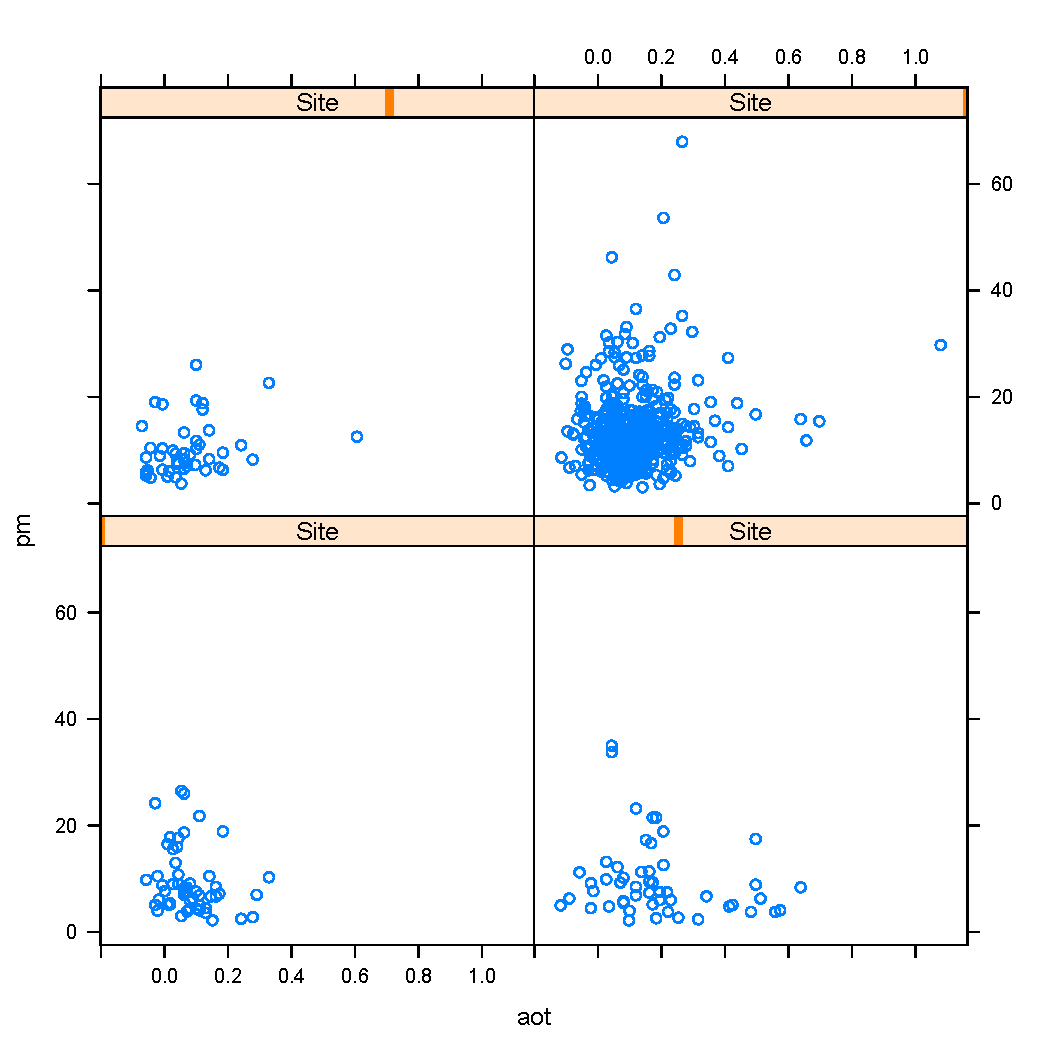
\includegraphics[width = 90mm]{3.pdf}
\caption{PM vs. AOD for the 4 west coast sites}
\label{fig:pm_vs_aod_west_four}
\end{figure}

Table \ref{variable_table} is notations for all the variables we used. 

\begin{table}[H] 
\centering
\begin{tabular}{|c|c|c|}
\hline
Variable & Description \\ 
\hline
$PM$ & Particulate Matter \\
$AOD$ & Aerosol Optical Depth \\
$U$ & Wind Speed \\
$V$ & Wind Direction \\
$H$ & Relative Humidity \\
$temp$ & Air Temperature \\
$se$ & Season (factor variable)\\
$si$ & Site (factor variable)\\
$d$ & Date (factor variable)\\
$ye$ & Year (factor variable)\\
\hline
\end{tabular}
\caption{Notations for variables}
\label{variable_table}
\end{table}

\subsubsection{Only AOD data}
Since there are many meteorological parameters varying from day to day, our statistical model must have the variability of the date. For each location, there are many different geographical properties, so our model must have the variability of sites. Therefore we used mixed effects model to fit this relationship:

$$PM_{ij} = \alpha + \beta\times AOD_{ij} + si_i + d_j+ \epsilon_{ij}, $$

where $PM_{ij}$ is the $PM_{2.5}$ concentration at a spatial site $i$ on a specific day $j$, $\alpha$ is the fixed intercept, $\beta$ is the fixed slope, $AOD_{ij}$ is the AOD value at a spatial site $i$ on a specific day $j$, $si_i\sim N(0, \sigma_s^2)$ is the random intercept of site $i$, $d_j\sim N(0, \sigma_d^2)$ is the random intercept of a specific day $j$, and $\epsilon_{ij}\sim N(0, \sigma^2)$ is the error term at site $i$ on a day $j$.

\subsubsection{AOD data and wind data}
As we have more information about the time-varying parameters, like air temperature, humidity, etc, it is not reasonable to simply treat them as a random variable. 

First, we tried the multivariate linear regression model to fit the relation. 

$$PM = \beta_0 + \beta_{AOD}\times AOD + \beta_{U}\times U + \beta_{V}\times V + \beta_{H}\times H + \beta_{temp}\times temp + se + ye\epsilon, $$
where $\epsilon\sim N(0, \sigma^2)$.

We also removed the outliers and did the stepwise regression to improve the model. 

But as the result of this model was still not good enough, we tried another
kind of model, the  Generalized Additive Model (GAM) model, which turned out to
be a better model to fit the relationship.




%\subsubsection{Match the AOD data with the PM$_{2.5}$ data}
%As we are trying to find the relationships between AOD and PM$_{2.5}$, we need
%to keep all the date the same, and locations closest. After matching these two
%datasets, we got the following as in table 2.~\alennote{Do you need this subsection?}
%\begin{table}[H]
%\centering
%\begin{tabular}{|c|c|c|c|c|c|c|}
%\hline 
%Date & lat\_pm & long\_pm & pm & lat\_aot & long\_aot & aot\\
%\hline
%2006-12-28 & 40.776944 & -124.1775 & 17.8 & 40.9 & -124.3 & 0.043815478682518\\
%\hline
%$\cdots$ & $\cdots$ & $\cdots$ & $\cdots$ & $\cdots$ & $\cdots$ & $\cdots$\\
%\hline
%\end{tabular}
%\caption{AOD and PM$_{2.5}$ match data}
%%%%%\label{}
%\end{table}





%%%%%%%%%%%%% 
\section{Computational Experiments}

\subsection{Experiment 1: Analysis of PM$_{2.5}$ time series}

\subsubsection{Holt-Winters Exponential Smoothing}
First we drew and plotted the fitted values based on Holt-Winters Exponential
Smoothing; see Figure 4, where the black line represents the variation of real PM$_{2.5}$ values
during 2004-2014 and the red line represents the variation of fitted PM$_{2.5}$ values
during the period. We can see that although the two lines have similar trends,
the fitted line is not accurate enough at many points.

\begin{figure}[H]
\centering
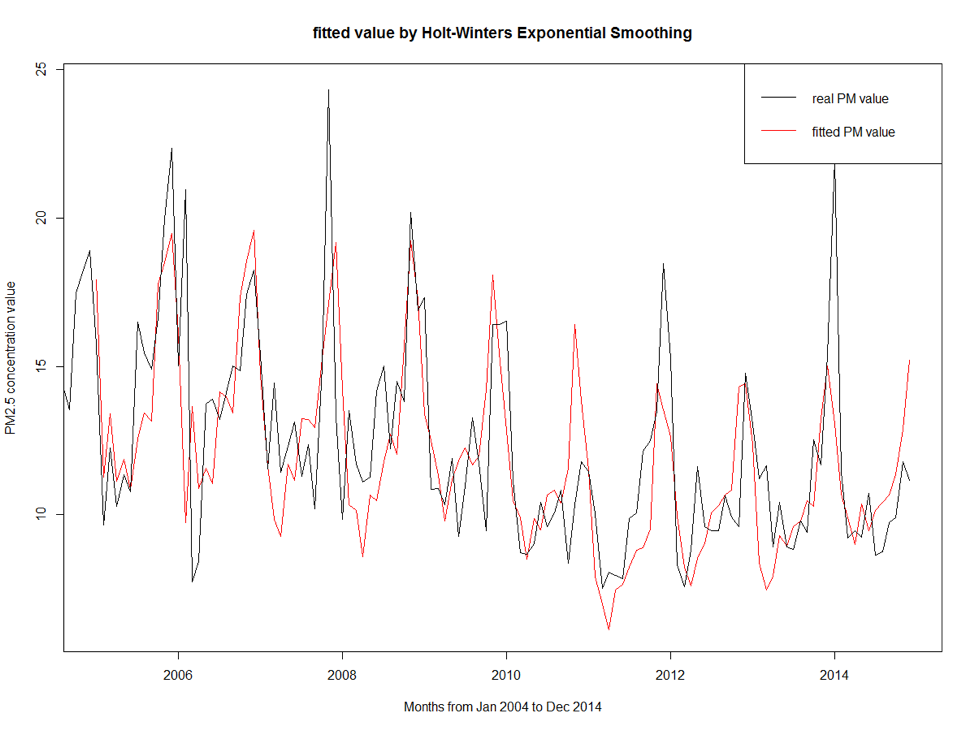
\includegraphics[width = 100mm]{ts2.png}
\caption{Fitted value by Holt-Winters Exponential Smoothing}
%\label{graph4}
\end{figure}

Next, we predict PM$_{2.5}$ values for the whole year 2015. In Figure 5, the
blue line represents the predicted values for 2015. The shadow of deep color
represents the 80\% prediction interval for the predicted values and the shadow
of light color represents the 95\% prediction interval for the predicted
values.

\begin{figure}[H]
\centering
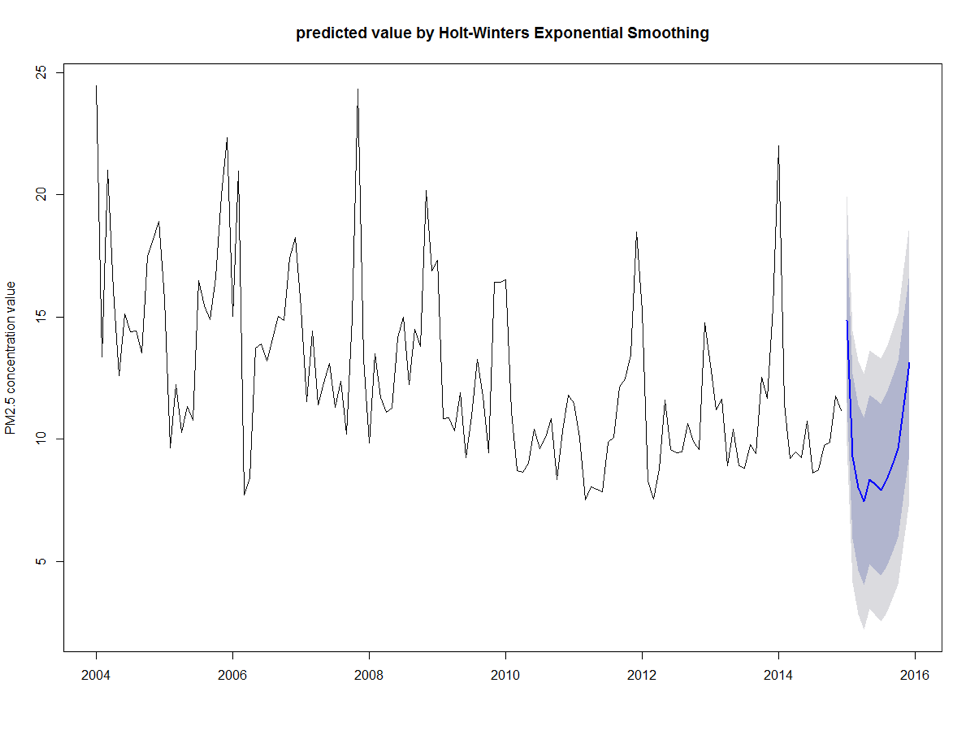
\includegraphics[width = 100mm]{ts3.png}
\caption{Predicted value by Holt-Winters Exponential Smoothin}
%\label{graph4}
\end{figure}

Lastly, we exmaine the effect of our prediction. We decide to use mean square
error as our criterion. Lower mean square error indicates we have a better
prediction. By comparing the predicted results and the real PM$_{2.5}$ values for the
year 2015, we find the mean square error between them is around 5.5. Because
the mean of PM$_{2.5}$ values during 2004-2014 is about 12.6, the mean square
error is too large to be acceptable and thus this model is not very accurate.

\subsubsection{ARIMA model}
Due to the seasonality in the PM$_{2.5}$ time series, we
want to decompose the time series and apply ARIMA model to the adjusted time
series. We firstly decompose the PM$_{2.5}$ time series and plot it. In Figure
6, the four subplots respectively represent observed values, overall trend
component, seasonal component and random part. From the seasonal component, we
can see that there does exist differences among PM$_{2.5}$ values in different
months. By subtracting the seasonal component from the original time series, we
get adjusted PM$_{2.5}$ time series.

\begin{figure}[H]
\centering
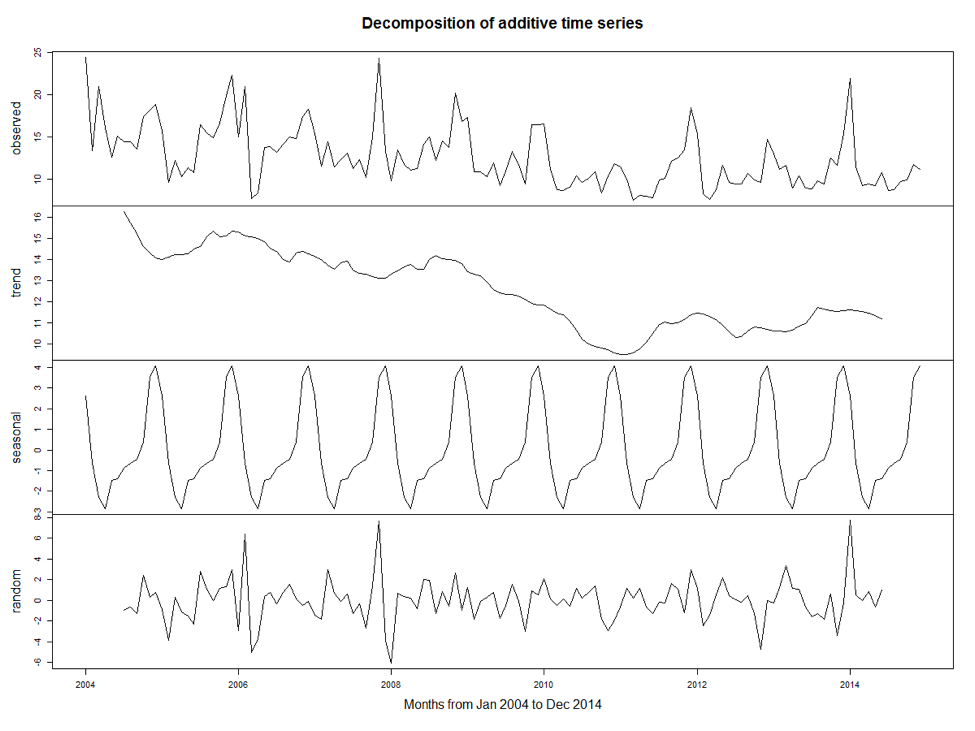
\includegraphics[width = 100mm]{ts4.png}
\caption{Decomposition of additive time series}
%\label{graph4}
\end{figure}

We then draw fitted adjusted PM$_{2.5}$ values based on ARIMA model in Figure 7. The
black line represents the variation of real adjusted PM$_{2.5}$ values during 2004-2014
and red line represents the variation of fitted adjusted PM$_{2.5}$ values during the
period. From this plot we can see that the fitted line is really rough.

\begin{figure}[H]
\centering
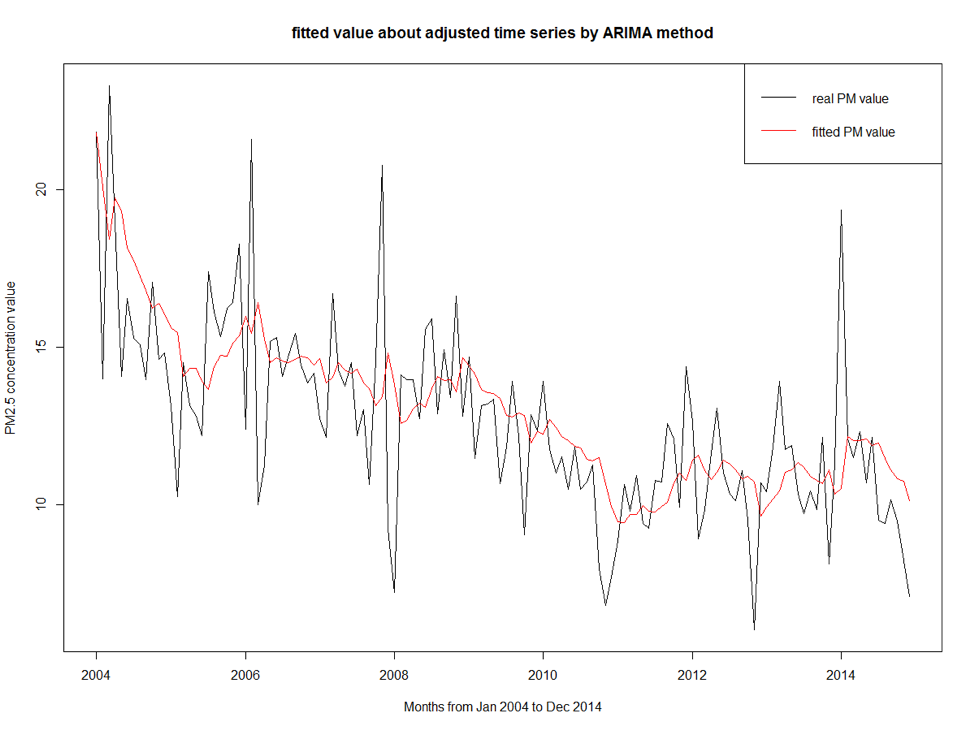
\includegraphics[width = 100mm]{ts5.png}
\caption{Fitted value about adjusted time series by ARIMA method}
%\label{graph4}
\end{figure}

Next, we predict the adjusted PM$_{2.5}$ values for the whole year 2015. In Figure 8, similarly as before, the blue line represents the predicted values for 2015. The shadow of deep color represents the 80\% prediction interval for the predicted values and the shadow of light color represents the 95\% prediction interval for the predicted values.

\begin{figure}[H]
\centering
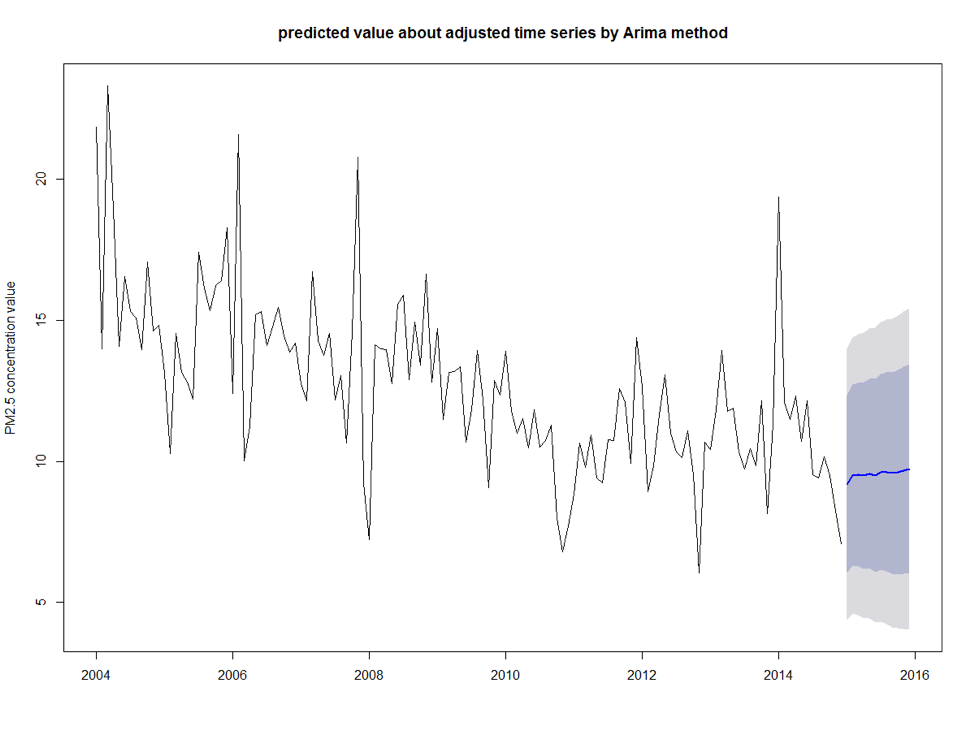
\includegraphics[width = 100mm]{ts6.png}
\caption{Predicted value about adjusted time series by Arima method}
%\label{graph4}
\end{figure}

Finally, we add seasonal component to our predicted results and then compare
them with the real PM$_{2.5}$ values during 2015. We find the mean square error is
around 9.7 so we believe the performance of ARIMA model is worse than 
Holt-Winters Exponential Smoothing.

In summary, the effect of prediction by time series is not very good, but it
does give us some inspirations. For example, the PM$_{2.5}$ values are different in
different seasons. The next analytical step,  will be to combine PM$_{2.5}$
values and some other corvariates to construct a better model.

%%%%%%%%%%%%
\subsection{Experiment 2: PM$_{2.5}$ vs AOD data}

Our main goal for experiment 2 is to explore the relationship between PM$_{2.5}$ measurements obtained from the ground sites and the AOD measurements obtained from the satellite near the coast. We want to ascertain whether satellite remote sensing can be used to assess PM$_{2.5}$ air quality for areas where surface PM$_{2.5}$  monitors are not available. The AOD measurements reflect the integrated amount of particles in the vertical column, and can be used as an input parameter in statistical models for predicting PM$_{2.5}$ levels. Since time-varying parameters such as relative humidity, wind direction, wind speed and air temperature can influence the PM$_{2.5}$-AOD relationship, we want to formulate a statistical model that allows for day-to-day variability in this relationship.  

We took notice from Figure \ref{fig:pm_vs_aod_four_west} that there was a huge difference between the $4$ sites we identified along the West Coast, so we decided to either treat the $site$ variable as a factor or build the model for each site along the West Coast. 

\begin{figure}[!h]
\centering
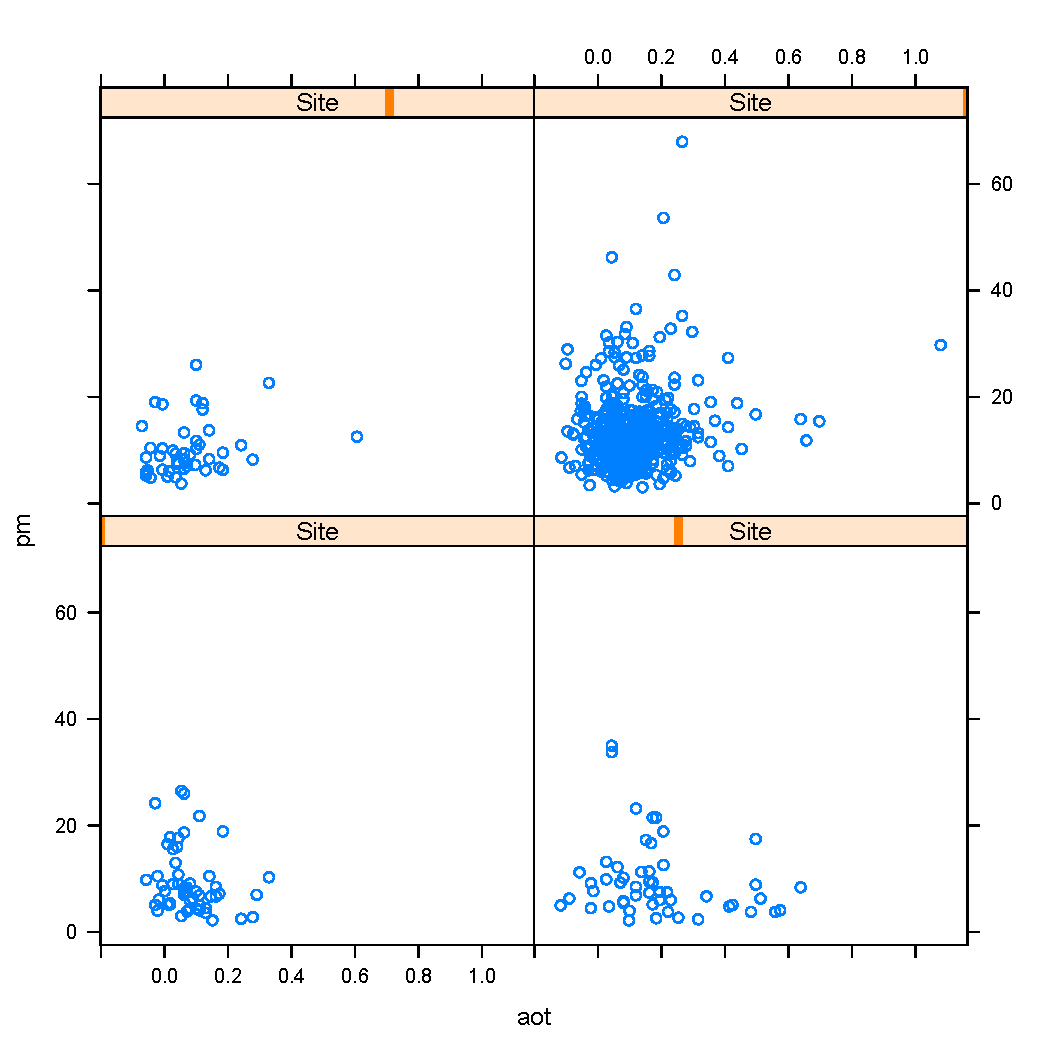
\includegraphics[width = 90mm]{3.pdf}
\caption{PM$_{2.5}$ vs. AOD for the 4 west coast sites}
\label{fig:pm_vs_aod_four_west}
\end{figure}

Table \ref{variable} refer to the  notations for all the variables we used. 

\begin{table}[H] 
\centering
\begin{tabular}{|c|c|c|}
\hline
Variable & Description \\ 
\hline
$PM$ & Particulate Matter \\
$AOD$ & Aerosol Optical Depth \\
$U$ & Wind Speed \\
$V$ & Wind Direction \\
$H$ & Relative Humidity \\
$temp$ & Air Temperature \\
$se$ & Season (factor variable)\\
$si$ & Site (factor variable)\\
$d$ & Date (factor variable)\\
$ye$ & Year (factor variable)\\
\hline
\end{tabular}
\caption{Notations for variables}
\label{variable}
\end{table}

subsection{Experiment 2: PM$_{2.5}$ vs AOD data}
\subsubsection{Only AOD data}
If we only use the AOD data, by using the approach in the Approach Section, we fitted the mixed effects model as follows.

$$\hat{PM}_{ij} = 10.51 + 3.60\times AOD_{ij} + \hat{si}_i + \hat{d}_j, $$

where $\hat{si}_i\sim N(0, 1.79^2)$ and $\hat{d}_j\sim N(0, 3.04^2)$. 

The correlation between the fitted PM$_{2.5}$ data and the true PM$_{2.5}$ data is 0.802, and $R^2 = 0.64$, which we agreed it is not a bad fit. 

\subsubsection{AOD data and wind data}
\paragraph{Multivariate linear regression model}

If we use both the AOD data and the wind data, as we mentioned in the Approach Section, we first tried to build a multivariate linear regression model. 

The following analysis is for the site (40.80178, -124.1621) and its  relation is different than for the sites mentioned in Section 3. For other sites, analysis should be similar. 

$$\hat{PM} = -0.64 - 0.0176\times AOD - 0.11\times U + 0.45\times V + 0.017\times H - 0.16\times temp + se + ye, $$

$R^2 = 0.758$.

\begin{figure}[H]
\centering
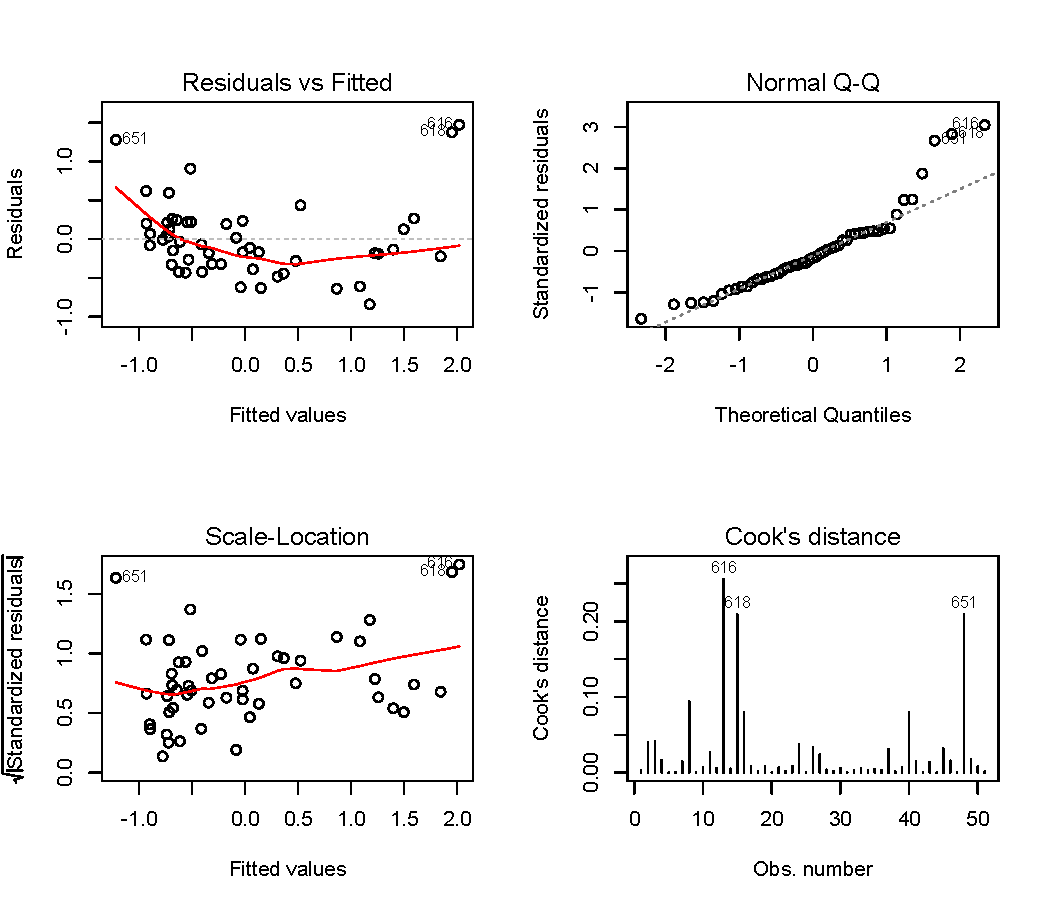
\includegraphics[width = 100mm]{residual.pdf}
\caption{Diagnosis 2}
\label{d1}
\end{figure}

We can see from figure \ref{d1} that there are three outliers. After deleting these outliers, the model became:

$$\hat{PM} = 94.43 + 2.34\times AOD - 1.11\times U + 0.033\times V - 0.068\times H - 0.30\times temp + se + ye, $$

$R^2 = 0.822$.

Then we did the stepwise regression to choose the best subset of all the variables, and got the following model:

$$\hat{PM} = 3.42 -1.07\times U + 0.036\times V+ se, $$
$R^2 = 0.786$.

\begin{figure}[H]
\centering
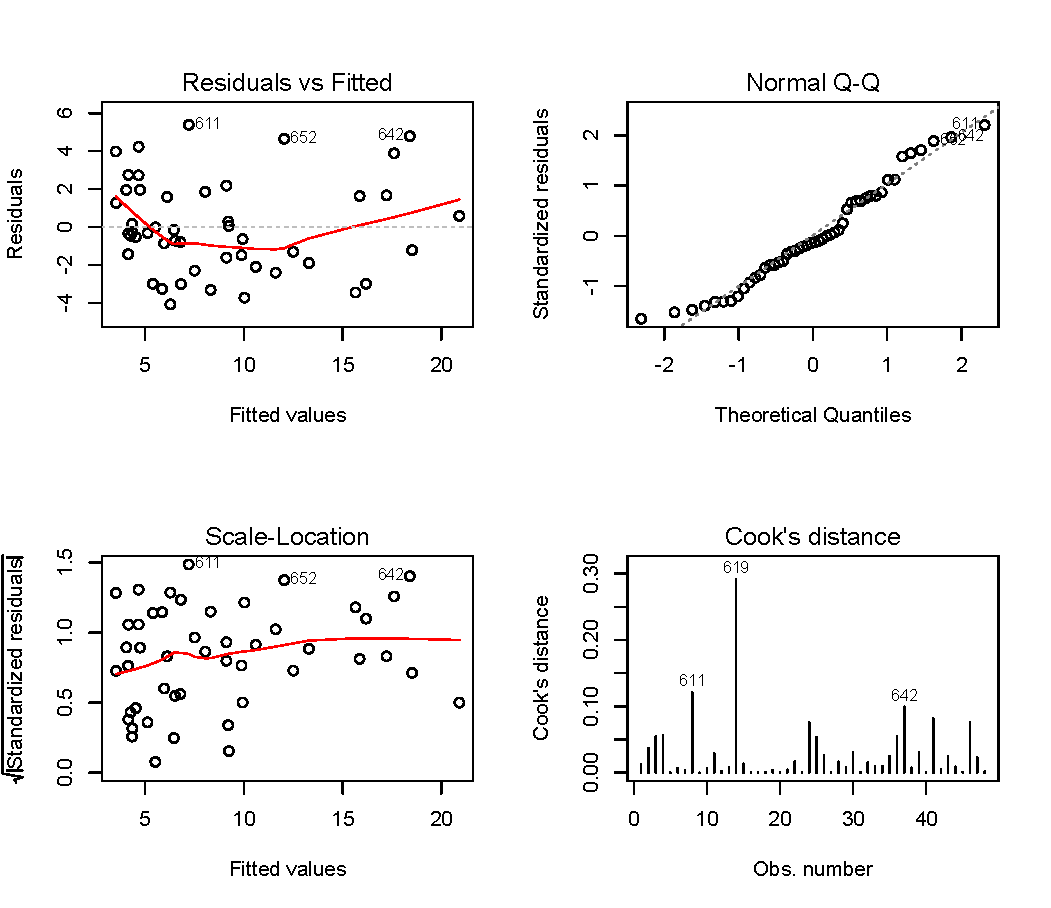
\includegraphics[width = 100mm ]{residual2.pdf}
\caption{Diagnosis 2}
\label{d2}
\end{figure}

Figure \ref{d2} are the diagnosis plots for the new model. Results obtained here were better than the previous model. But we can see from those plots that the residuals still have some trend and some cluster, which shows that this model violated some assumptions, like the equal variance assumption for the linear regression model. To figure out if this model is good, we did 5-fold cross validation. The results are described in figure \ref{cv}. 

\begin{figure}[H]
\centering
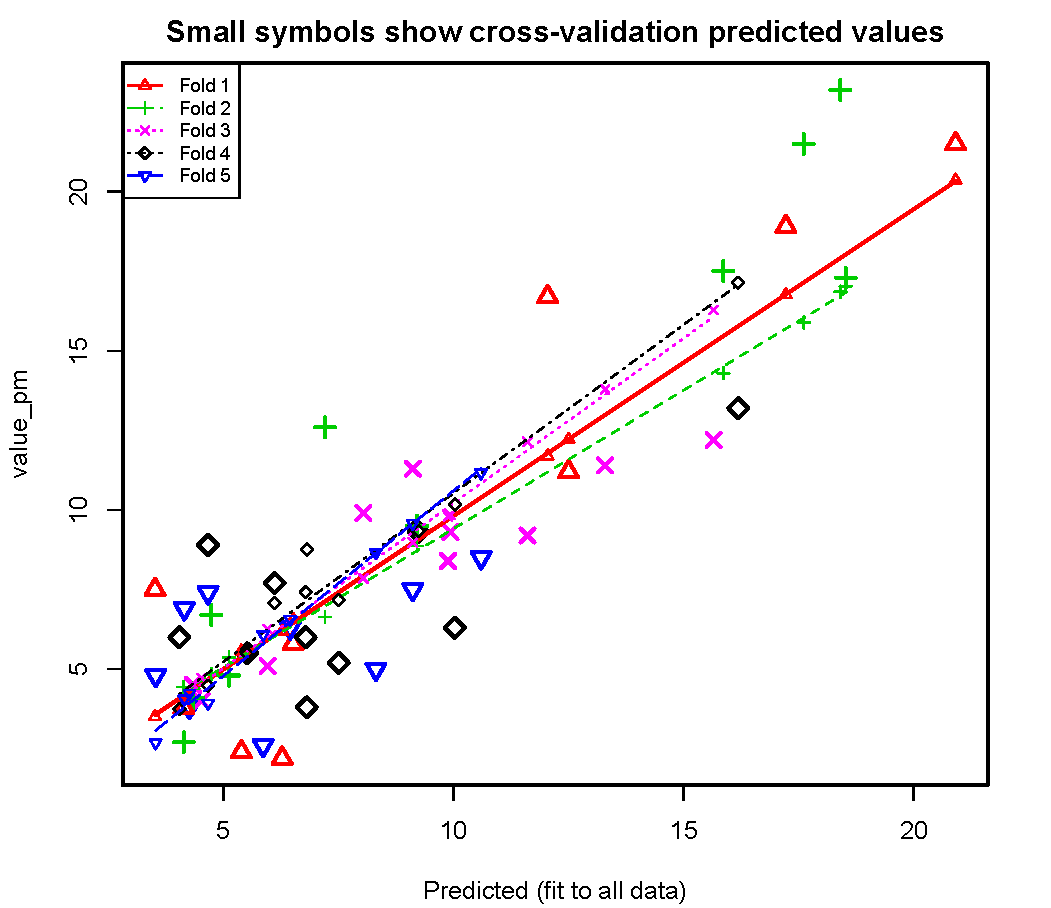
\includegraphics[width = 100mm]{cv_lm.pdf}
\caption{5-fold cross validation for the multivariate linear regression model}
\label{cv}
\end{figure}

The mean square error for cross validation is 8.16. As the average PM$_{2.5}$ values is 8.75, 8.16 is pretty high as there would be $\frac{\sqrt{8.16}}{8.75}=32.65\%$ error for PM$_{2.5}$ value, which is high. Another reason that we agreed this is not a good model is that it actually did not include the AOD data as predictors. According to the meteorologic knowledge, AOD should play a key role in the model. Above all, we concluded that the multivariate linear regression model is not good.

\paragraph{GAM model}

An appropriate initial model structure would probably involve modeling PM$_{2.5}$ as a linear/non-linear function of the AOD measurements and other aforementioned time-varying parameters,but before attempting to fit the models, it is worth examining the data itself to look for possible problems. When this is done, AOD measurements with values $< -0.05$ appear problematic since AOD values are usually constrained to lie between 0 and unity. For this reason, these values are excluded from the analysis. 

\begin{figure}[H]
\centering
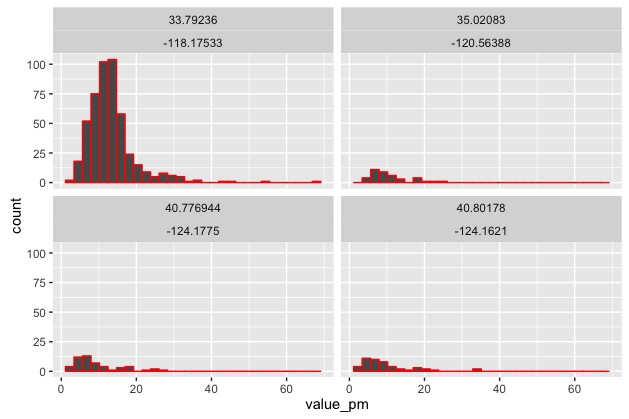
\includegraphics[width=100mm]{histpmcali.jpeg}
\caption{Histograms for PM$_{2.5}$ measurements at 4 sites in California. The titles on each subpanel represent the latitudes and longitudes for the sites respectively.}
\end{figure}

The fairly skewed nature of the PM$_{2.5}$ measurements, the response, and the fact that it is necessarily a positive quantity, suggest that some transformation maybe required if a Gaussian error model is to be used. Attempting to use a Gaussian model without transformation confirms this. The upper left normal QQ plot, in figure 15, clearly shows a problem with the Gaussian assumption. Examining the plot on upper right of residuals versus fitted values reveals that the constant variance assumption is unreasonable. The lower left histogram of residuals confirms the pattern evident in the QQ plot: there are too many residuals in the lower tail which means that we tend to over estimate the PM$_{2.5}$ levels using the model. The lower right plot emphasizes the failure of the constant variance assumption. \\ From figure 15, it is difficult to guess the appropriate transformation on the PM$_{2.5}$ measurements that would alleviate this issue. We explored two options. Fitting the log transformation of the PM$_{2.5}$ variable to the data tell the same story and, as before, runs into similar problems like non-constant variance and an unreasonable Gaussian assumption. The residual plots are not shown here.

\begin{figure}[H]
\centering
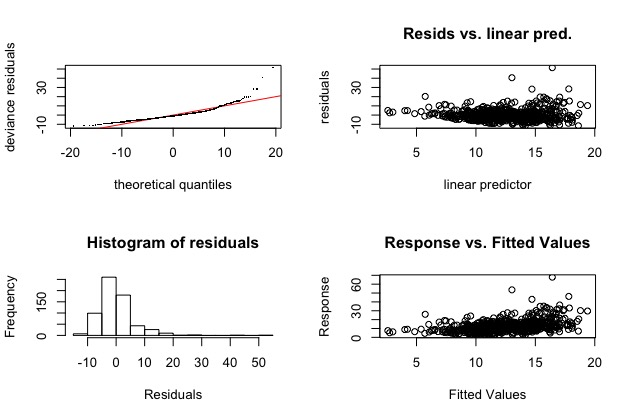
\includegraphics[width=0.8\textwidth]{gauss_diag.jpeg} 
\caption{Some basic model checking plots for a model fitted to the PM$_{2.5}$ - AOD data} 
\end{figure}


Generalized Additive Models (GAMs) employ a class of equations called "smoothers" or "scatterplot smoothers" that attempt to generalize data into smooth curves by local fitting to the subsections of the data. The basic idea behind GAMs can be described as follows. We calculate a smooth curve that goes through the data as well as possible while being parsimonious. Note that it is possible using a polynomial of high enough order to get a curve to go through every point. This makes the curve "wiggle" excessively, and not represent a parsimonious fit. The approach generally employed with GAMs is to divide the data into some number of intervals/sections, using "knots" as the end points of these intervals. Then a low order polynomial or spline function is to fit the data in an interval, with the added constraint that the second derivative of the function at the knots must be the same for both intervals sharing the knot. This eliminates sharp edges in the curve, and ensures that it is smooth and continuous at all points. As a practical matter, we can view GAMs as non-parametric curve fitters that attempt to achieve an optimal compromise between goodness-of-fit and parsimony of the final curve. One of the interesting aspects of GAMs is that they can only approximate the appropriate number of degrees of freedom, and that the number of degrees of freedom is often not an integer, but rather a real number with some fractional component. A second order polynomial (or quadratic equation) in a GLM uses two degrees of freedom (plus one for the intercept). A curve that is slightly less regular than a quadratic might require two and a half degrees of freedom (plus one for the intercept), but might fit the data better. The other aspects of GAMs that is different is that they don't handle interaction well. Rather than fit multiple variables simultaneously, the algorithm fits a smooth curve to each variable seperately and then combines the results additively, thus giving rise to the name Generalized Additive Models~\cite{GAM_ref}.

We model the variability in $\PM$ concentrations using generalized additive models (GAMSs) (Hastie and Tibshirani 1990). Our model can be described as follows, 
\begin{equation} 
{\mathbb{E}}(Y_{t,site} \mid AOD, U, V, H, temp, Season) = \beta_0 + \text{AOD} + f_{U}(U) + f_{V}(V) + f_{H}(H) + f_{temp}(temp) + \text{Season}  
\end{equation} 
$Y_{t, \text{site}}$ is the daily $\PM$ concentration at a given site. All the covariates vary with time and site. $\mu$ is the random model intercept, $f_{U}(U)$, $f_{V}(V)$ are one dimensional smooth surfaces describing the impact of wind speed and direction on the AOD-$\PM$ association. Season is modeled as a 4-level categorical variable because of its discrete values. \\ \\
We fit the model with the $gam()$ function in the {\textit{mgcv}} package in R (Wood 2006). The package ${mgcv}$ uses penalized regression splines for the $f_{j}$, so we can write
\begin{center} 
$f_{j}(x) = \sum \beta_{jk} {\phi_{jk}}(x) = {\bm{\beta{'}}}{\phi_j}$
\end{center} 
for the basis functions ${\phi_{jk}}$ that determine the splines. Given the basis function representation of the $f_j$, (1) is now a parametric mean function with parameters 
${\bf{\beta}} = (\beta_0, {\bm{\beta}_1'}, \ldots, {\bm{\beta}_n'})'$ 
and predictors that define the intercept and the splines that define the $s_j$.  \\
The penalized least squares objective function for estimating ${\bm{\beta}}$ is 
\begin{equation} 
{\lVert Y - X{\bm{\beta}}\rVert}^{2} + \sum_{j}\lambda_{j}{\bm{\beta}_j'}{\bm{\beta}_j}
\end{equation}
The values of $\lambda_{j}$ are selected in an iterative algorithm to minimize a generalized cross validation criterion. This fit is done using the ${gam}$ function in the ${mgcv}$ package, 
\begin{verbatim}
Family: gaussian 
Link function: identity 

Formula:
value_pm ~ (value_aod) + s(windirection) + s(hum) + s(airtemp) + 
    season

Parametric coefficients:
            Estimate Std. Error t value Pr(>|t|)    
(Intercept)    4.085      1.065    3.84  0.00023 ***
value_aod     -2.283      2.330   -0.98  0.32993    
season         2.485      0.384    6.47  5.2e-09 ***
---
Signif. codes:  0 ‘***’ 0.001 ‘**’ 0.01 ‘*’ 0.05 ‘.’ 0.1 ‘ ’ 1

Approximate significance of smooth terms:
                 edf Ref.df     F p-value    
s(windirection) 2.66   3.28 35.38 < 2e-16 ***
s(hum)          2.46   3.00  1.37 0.24676    
s(airtemp)      3.07   3.81  5.73 0.00051 ***
---
Signif. codes:  0 ‘***’ 0.001 ‘**’ 0.01 ‘*’ 0.05 ‘.’ 0.1 ‘ ’ 1

R-sq.(adj) =  0.786   Deviance explained = 80.8%
GCV = 11.065  Scale est. = 9.8282    n = 100
\end{verbatim} 
The only visible parameter in this model is the intercept, estimated to be 4.085. The ${\bm{\beta_{j}}}$ are hidden inside the smoothers and are largely uninterpretable. For each of its predictors, a smoother was fit by the $f$ functions. The default in the function $f$ that does the smoothing uses {\textit{thin plate regression splines}} that don't depend as much on the number of knots selected and also they generalize to smooths of more than one variable at a time. In the output, the "edf" is the equivalent degrees of freedom for each of the smooths. If we are using $k$ basis functions for a smooth, then we would have $k$ degrees of freedom (df) for the smooth. Penalization will generally reduce edf to a number smaller than $k$. The adjusted $R^{2}$ is the square of the correlation between the observed and fitted values, with an adjustment for degree of freedom, while the deviance explained appears to be the usual $R^2$. 



\begin{figure}[h]

\centering
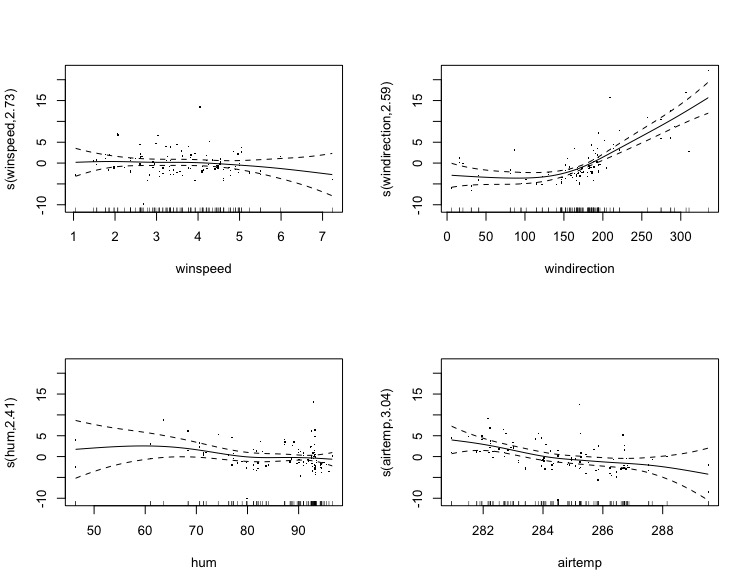
\includegraphics[width=0.8\textwidth]{pred.jpeg} 
\caption{The estimates of the smooth functions shown without partial residuals. We plot two times the standard errors of the estimates (in dashed lines).} 
\end{figure} 
In Figure 4, the solid line is the predicted value of the dependent variable as a function x axis. We plot two times the standard errors of the estimates (in dashed lines). The small lines along the x axis are the "rugs" showing the location of the sample plots. The result for all the predictors look relatively flat because the standard errors are not too large. \\ 
We also perform the likelihood ratio tests to compare different models and conclude that the model displayed on the previous page does the best job. 












\subsection{Experiment 3: Spatial Statistics}
In this section, we build spatial models for the AOD and PM$_{2.5}$ data. In spatial
statistics, we study the relations and variation in data with respect to its
location. Spatial statistics on a geological set is carried out in two stages:

\begin{itemize}
\item Analyze the dataset to build a relation (covariance) amongst values based
on their geographical location. In the language of statistics, this means
building a variogram which models variance between values at two locations
according to the distance and direction between them.

\item The next step is to estimate values at unsampled locations via 
the process of ``Kriging''. The interpolated values obtained by Kriging are modeled
using a Gaussian process directed by prior covariances. Note that in contrast to Kriging,
using polynomial interpolation optimizes the smoothness of the interpolated values.  

\end{itemize}

We use ordinary Kriging to interpolate AOD and PM$_{2.5}$ values. In ordinary
Kriging, the interpolated value is a weighted linear combination of sampled
values. Ordinary Kriging assumes a constant mean and residual mean error of 0.
Along with this, ordinary Kriging aims to minimize the variance of error. The
variogram gives the covariances between different values. Ordinary Kriging is
obtained by using probability models that calculate the bias and error in
variance, which can then be used to choose weights for neighboring sampled
locations such that mean error for the model is exactly zero and modeled error
variance is minimized. We have used a maximum likelihood probability model to
estimate parameters. We obtain the spatial plots and standard error associated
with the interpolations using this method of Kriging. 

There are $284$ sensor sites that recorded the PM$_{2.5}$ measurements. We use
the daily  PM$_{2.5}$ measurements at these sites to make spatial interpolation
plots. Similarly, spatial interpolation plots are constructed for AOD values.
Figure \ref{aodpm}(left)  below displays the 107 sensor sites where PM$_{2.5}$ data
was collected on 7th January, 2009. 

\begin{figure}[H]
\centering
  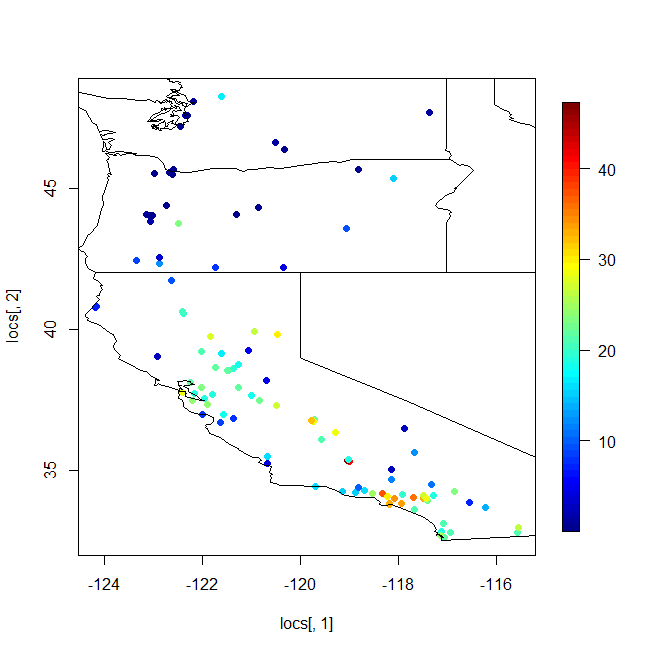
\includegraphics[width=.45\textwidth]{SamplePoints07012009.png}
  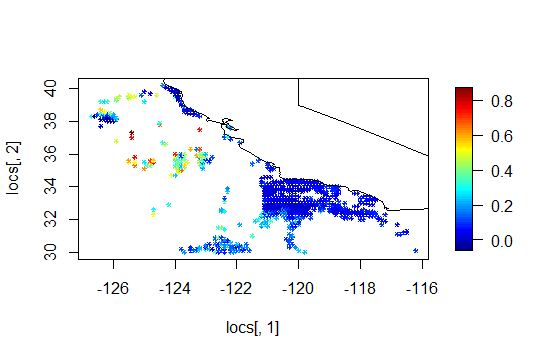
\includegraphics[width= .45\textwidth]{AODpoints_06012009.png}
  \caption{Left: January 7, 2009 PM$_{2.5}$ sites; right: January 6, 2009 AOD sites.}
\label{aodpm}
\end{figure}


Figure~\ref{examplepm} displays the spatially interpolated plot obtained by
using ordinary Kriging of the sample data and the standard error associated
with the interpolated values. As expected, we see the error increases as
distance from the sample data increases. 

\begin{figure}[H]
\centering
  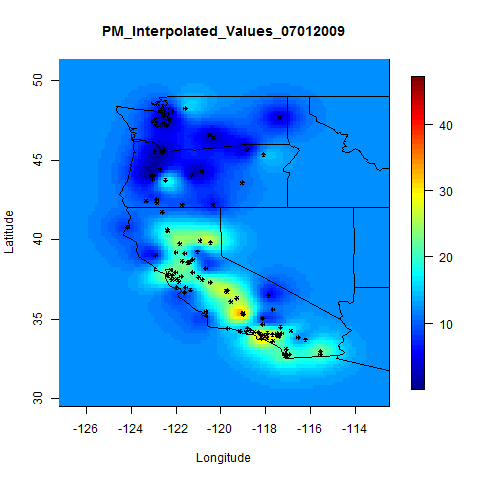
\includegraphics[width=0.45\textwidth]{Interpolated_PM2009_0007.png}
  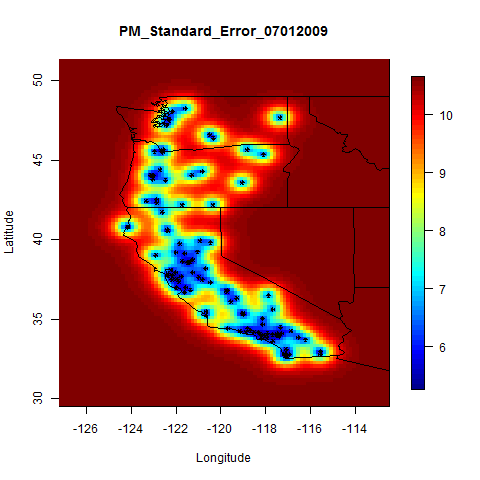
\includegraphics[width=0.45\textwidth]{Standard_Error_PM2009_0007.png}
  %\label{fig:sub2}
%  \caption{January 7, 2009}
%  \caption{ Interpolated PM$_{2.5}$ with ordinary kriging}
  \caption{January 7, 2009. Left: Interpolated PM$_{2.5}$ with ordinary kriging; right: 
standard error associated with the interpolated PM$_{2.5}$ values.}
\label{examplepm}
\end{figure}

\begin{figure}[H]
\centering
  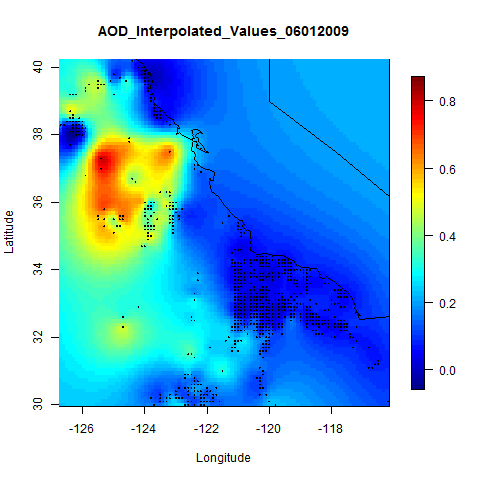
\includegraphics[width=.45\textwidth]{Interpolated_AOD2009_06.png}
  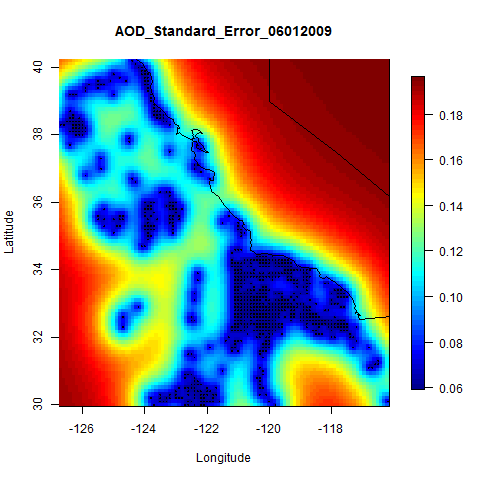
\includegraphics[width=.45\textwidth]{StandardError_AOD2009_06.png}
\caption{January 6, 2009. Left: Interpolated AOD with ordinary kriging; right: 
standard error associated with the interpolated AOD values.}
\label{exampleaod}
\end{figure}


Similarly, we construct spatially interpolated plots for AOD data obtained on
6th January, 2009. Figure~\ref{aodpm}(right) displays sites where AOD was measured.
Figure \ref{exampleaod} displays the spatially interpolated plot obtained by
using ordinary Kriging of the sample AOD data and the error associated with the
interpolated values.

\begin{figure}[H]
\centering
  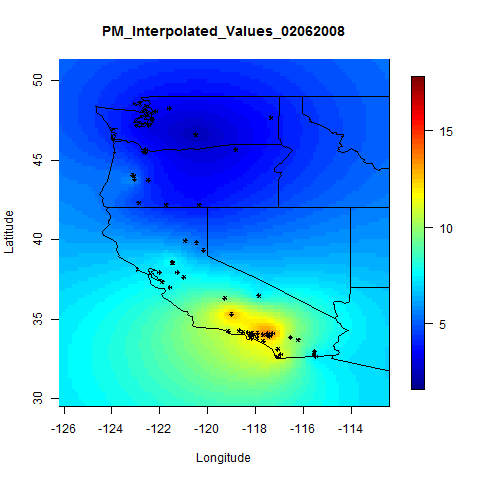
\includegraphics[width=0.45\textwidth]{Interpolated_PM2008_0154.png}
  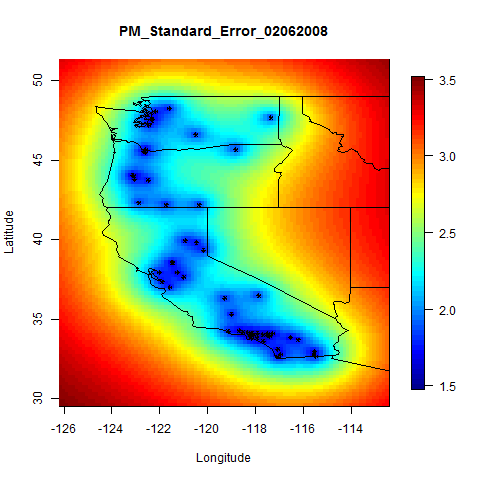
\includegraphics[width=0.45\textwidth]{Standard_Error_PM2008_0154.png}
\caption{June 2, 2008.  Left: Interpolated PM$_{2.5}$ with ordinary kriging; right:
standard error associated with the interpolated PM$_{2.5}$ values.}
\label{normalday}
\end{figure}

The Basin Complex wildfire in Monterey County California started on 21 June,
2008 and was contained by 27 July, 2008. One of the most common causes of
PM$_{2.5}$ is wildfires. Hence, we expect to observe higher PM$_{2.5}$
concentrations in the central coast during that time period. In Figure
\ref{normalday}, we have spatial plots for PM$_{2.5}$ on 2nd June, 2008. We see
that, on a normal day, PM$_{2.5}$ concentration is high around Los Angeles. We
see this pattern of higher PM$_{2.5}$ concentration around Los Angeles
consistently in our dataset.  More broadly, according to a study, Los Angeles
is the most polluted city in California, thus the PM$_{2.5}$ match with our
expectations~\cite{fire3}.



To trace the special case of a wildfire, we observe PM$_{2.5}$ spatial plots
over the western states of U.S. from 27th June to 30th June 2008 Figure
\ref{june27}, Figure \ref{june28}, Figure \ref{june29}, and Figure \ref{june30}.
Here, we observe the PM$_{2.5}$ concentration is higher in northern California,
significantly more so than even the Los Angeles sites on these dates. Following
the spatial plot over 4 days, we can notice PM$_{2.5}$ region with higher
concentration to be moving towards the north. These plots verify the presence
of a wildfire and the spatial plots over time suggest the direction of movement
of the smoke produced due to the wildfire. 

%%%June 27, 2008
\begin{figure}[H]
\centering
  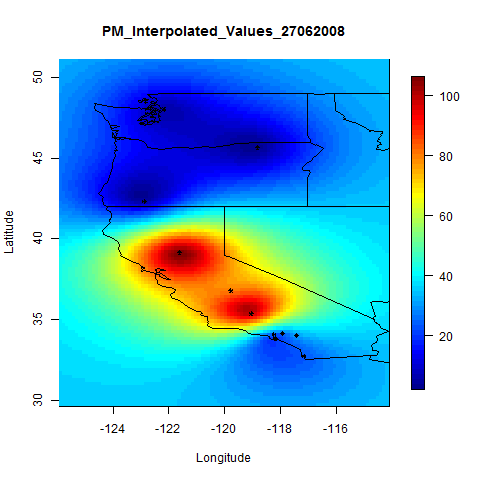
\includegraphics[width=.45\textwidth]{Interpolated_PM2008_0179.png}
  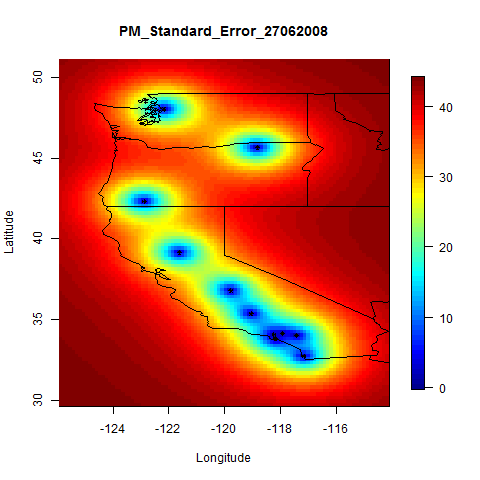
\includegraphics[width= .45\textwidth]{Standard_Error_PM2008_0179.png}
\caption{June 27, 2008.  Left: Interpolated PM$_{2.5}$ with ordinary kriging; right:
standard error associated with the interpolated PM$_{2.5}$ values.}
\label{june27}
%  \label{june27:sub1}
\label{june27:sub2}
\end{figure}

%%%%%June 28, 2008
\begin{figure}[H]
\centering
  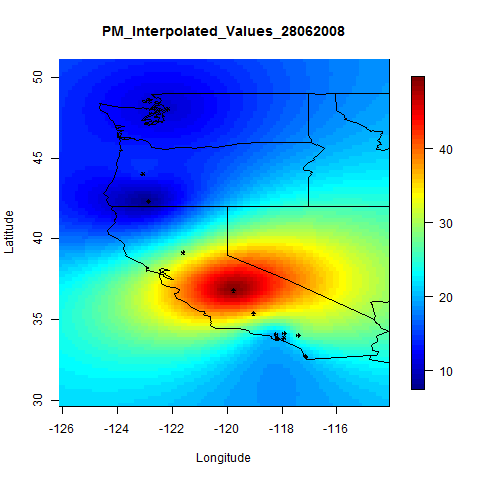
\includegraphics[width=.45\textwidth]{Interpolated_PM2008_0180.png}
  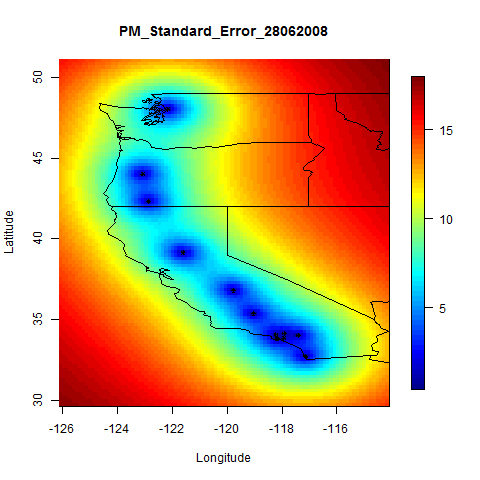
\includegraphics[width= .45\textwidth]{Standard_Error_PM2008_0180.png}
\caption{June 28, 2008.  Left: Interpolated PM$_{2.5}$ with ordinary kriging; right:
standard error associated with the interpolated PM$_{2.5}$ values.}
  %\label{june28:sub1}
  %\label{june2008:sub2}
\label{june28}
\end{figure}

%%%%%%%%June 29, 2008
\begin{figure}[H]
\centering
  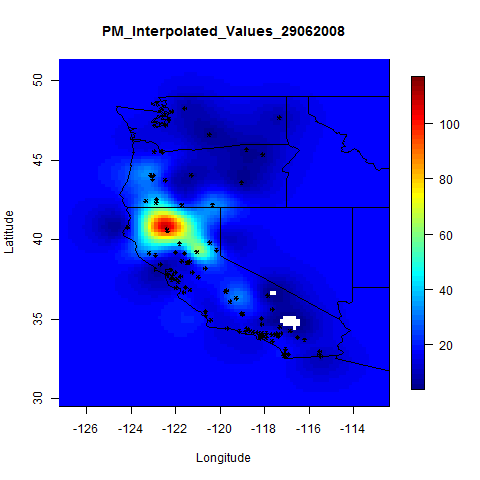
\includegraphics[width=.45\textwidth]{Interpolated_PM2008_0181.png}
  %\label{fig:sub1}
  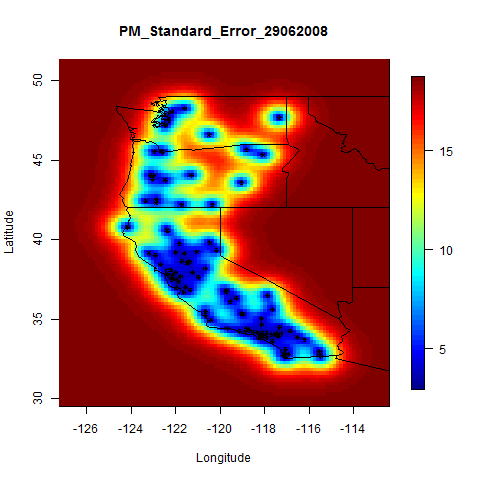
\includegraphics[width= .45\textwidth]{Standard_Error_PM2008_0181.png}
  %\label{fig:sub2}
\caption{June 29, 2008.  Left: Interpolated PM$_{2.5}$ with ordinary kriging; right:
standard error associated with the interpolated PM$_{2.5}$ values.}
\label{june29}
\end{figure}

%%%%%%%%%%June 30, 2008
\begin{figure}[H]
\centering
  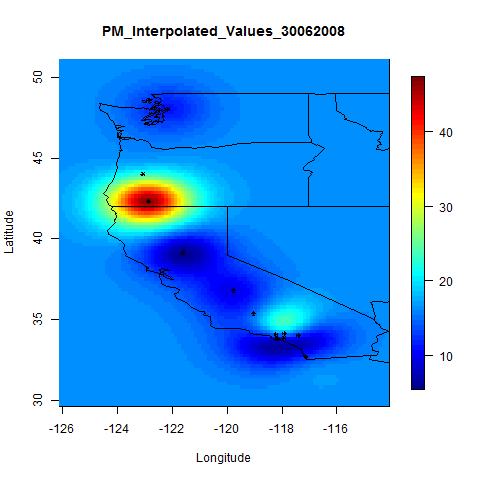
\includegraphics[width=.45\textwidth]{Interpolated_PM2008_0182.png}
  %\label{fig:sub1}
  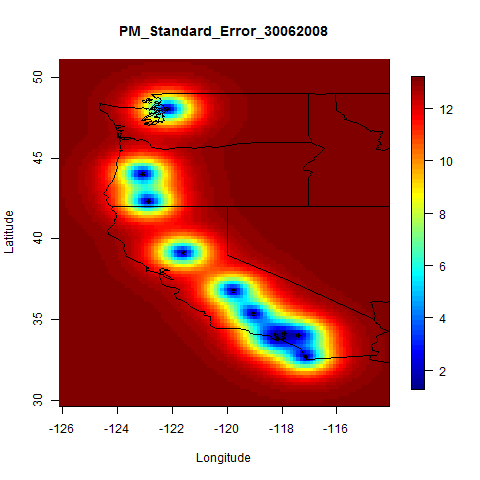
\includegraphics[width= .45\textwidth]{Standard_Error_PM2008_0182.png}
  %\label{fig:sub2}
\caption{June 30, 2008.  Left: Interpolated PM$_{2.5}$ with ordinary kriging; right:
standard error associated with the interpolated PM$_{2.5}$ values.}
\label{june30}
\end{figure}


In future work, we plan to verify our results by comparing our observations with the a
different satellite data and/or satellite images over that period. This example
suggests that by studying the spacial model over time, we can trace the
movement of high volumes of PM$_{2.5}$.



\section{Summary and Future Work}
\subsection{Summary}

We can see that the mixed effects model which uses only the AOD data has
the lowest $R^2$. If both the AOD data and the meteorological information are
used, multivariate linear regression model works better than if we only use the
AOD data. But it violates the equal variance and normal distribution assumption
from the diagnosis plots. Overall, GAM model works much better than the
multivariate linear regression model.

We can conclude from our GAM model that the satellite measurements (AOD)
have a linear relationship with the PM$_{2.5}$ measurements while the other
meteorological variables have a non-linear relationship with PM$_{2.5}$. Trying
to model the relationship by combining different sites together affects the
performance of the model drastically. We recommend building a separate model
for every site in order to tackle this issue.


We analyze PM$_{2.5}$ time series to see whether previous PM$_{2.5}$ values can
be used to predict future values.  We apply Holt-Winters Exponential Smoothing
and ARIMA method to monthly average PM$_{2.5}$ values from 2004-2014 and then
make a prediction about PM$_{2.5}$ values in 2015. Comparing predicted results
with the real PM$_{2.5}$ values in 2015, we find the prediction effects of
these two methods are not good enough. Thus, we believe predicting future
PM$_{2.5}$ values by itself in not a good idea and we should combine more
covariates in our model.  

\subsection{Future Work}

\begin{itemize}
\item We would like to incorporate Hawaii sites to build the statistical model
for predicting PM$_{2.5}$ using AOD measurements. Since Hawaii is surrounded by
ocean,  the GAM model that works well in west coast data may not perform well. 
One could also explore different models to see if there is any better model than the GAM.

\item We would also like to make our model robust by training the data over
several years.  We used 2006-2009 data in this report. If we can use more data,
for example, 2000-2009, the model would be more accurate.

\end{itemize}





%\section{Summary and Future Work}
%\subsection{Summary}
%
%\subsection{Future Work}
%Undoubtedly, there is a lot of work to be done further. Firstly, we would like to incorporate Hawaii sites to make the statistical model for predicting PM$_{2.5}$ using AOD measurements. Hawaii islands  are We would like make our model robust by training the data over several years.  We aim to make PM$_{2.5}$ predictions over the ocean using this model. With the predicted PM$_{2.5}$ values, we would make spatial plots. Spatial variations observed over a a time scale can provide insightful information about  intercontinental movement of PM$_{2.5}$. 



 \begin{thebibliography}{99}
 
 \bibitem{noaa} National Centers for Environmental Information. National Oceanic and Atmospheric Administration. Department of Commerce, n.d. Web. 23 July 2016. \textit{https://www.ncdc.noaa.gov/cdr/atmospheric/avhrr-aerosol-optical-thickness}.
 
 \bibitem{epa} United States Environmental Protection Agency. AirData. EPA, 5 July 2016. Web. 23 July 2016. \textit{https://www3.epa.gov/airdata/}.
 
 \bibitem{liu} Liu, Yang, Christopher J. Paciorek, and Petros Koutrakis. \textit{Estimating Regional Spatial and Temporal Variability of PM$_{2.5}$ Concentrations Using Satellite Data, Meteorology, and Land Use Information.} 6th ed. Vol. 117. N.p.: Environmental Health Perspectives, June 2009. Print.
 
 \bibitem{lee} Lee, H J., Y Liu, B A. Coull, J Schwartz, and P Koutrakis. \textit{A novel calibration approach of MODIS AOD data to predict PM$_{2.5}$ concentrations.} N.p.: Atmospheric Chemistry and Physics, 2011. Print.
 
 \bibitem{donk} Donkelaar, Aaron von, Randall V. Martin, Michael Brauer, and Brian L. Boys. \textit{Use of Satellite Observations for Long-Term Exposure Assessment of Global Concentrations of Fine Particulate Matter.} 2nd ed. Vol. 123. N.p.: Environmental Health Perspectives, 2015. Web. 26 July 2016. \textit{http://dx.doi.org/10.1289/ehp.1408646}
 
 \bibitem{li} Li, Jing, Barbara E. Carlson, and Andrew A. Lacis. \textit{ How well do satellite AOD observations represent the spatial and temporal variability of PM$_{2.5}$ concentration for the United States?} N.p.: Atmospheric Environment, 2015. Print.
 
 \bibitem{nasa} \textit{Goddard Earth Sciences Data and Information Services Center.} NASA, n.d. Web. 26 July 2016. \textit{http://disc.sci.gsfc.nasa.gov/giovanni/additional/users-manual/}
 
 \bibitem{lam} \textit{Lambert Conformal Conic}. GeoReference, n.d. Web. 26 July 2016. \textit{http://www.georeference.org/doc/lambert\_conformal\_conic.html}
 
 \bibitem{wind} \textit{Earth Observing Laboratory.} NCAR UCAR, n.d. Web. 26 July 2016. \textit{https://www.eol.ucar.edu/content/wind-direction-quick-reference}
 
 
 \bibitem{fire1} \textit{Top 20 Largest California Wildfires.} Cal Fire, n.d. Web. 26 July 2016. \textit{http://www.fire.ca.gov/communications/downloads/fact\_sheets/20LACRES.pdf}
 
 \bibitem{fire2} Kenward, Alyson, Dennis Adams-Smith, and Urooj Raja. "WILDFIRES and AIR POLLUTION." Climate Central, 2013. Web. 26 July 2016. \textit{http://assets.climatecentral.org/pdfs/WildfiresAndAirPollution.pdf}
 
 \bibitem{fire3} "Most Polluted Cities." \textit{Sate of the Air}. American Lung Association, 2013. Web. 26 July 2016. \textit{http://www.stateoftheair.org/2013/city-rankings/most-polluted-cities.html?referrer=https://en.wikipedia.org/}
 
 
 
 \bibitem{littlebook} "Using R for Time Series Analysis." N.p., n.d. Web. 26 July 2016. \textit{http://littlebookofrtimeseries-zh-cn.readthedocs.io/en/latest/src/timeseries.html\#time-series-analysis}
 
 \bibitem{nist} "What is Exponential Smoothing? ." Engineering Statistics Handbook. N.p., n.d. Web. 26 July 2016. \textit{http://www.itl.nist.gov/div898/handbook/pmc/section4/pmc43.htm}
 
 \bibitem{wik} "Autoregressive integrated moving average." Wikipedia. N.p., n.d. Web. 26 July 2016. \textit{https://en.wikipedia.org/wiki/Autoregressive\_integrated\_moving\_average}
 
 
\bibitem{GAM_ref}
Course notes. Web. 27 July 2016.
\textit{ecology.msu.montana.edu/labdsv/R/labs/lab5/lab5.html}
 \end{thebibliography}

\end{document}
















